% ============================================================================
% Multi-Objective Optimization for Image Classification — Report
% ============================================================================
\documentclass[12pt, a4paper]{article}

% ---- Packages ----
\usepackage[utf8]{inputenc}
\usepackage[T1]{fontenc}
\usepackage{amsmath, amssymb, amsfonts}
\usepackage{graphicx}
\usepackage{booktabs}
\usepackage{hyperref}
\usepackage{geometry}
\usepackage{float}
\usepackage{caption}
\usepackage{subcaption}
\usepackage{algorithm}
\usepackage{algpseudocode}
\usepackage{xcolor}
\usepackage{listings}
\usepackage{enumitem}
\usepackage{tabularx}
\usepackage{multirow}
\usepackage{array}

\geometry{margin=2.5cm}
\hypersetup{colorlinks=true, linkcolor=blue!60!black, citecolor=green!50!black, urlcolor=blue!70!black}

% ---- Code listing style ----
\lstset{
    basicstyle=\ttfamily\small,
    keywordstyle=\color{blue!70!black}\bfseries,
    commentstyle=\color{green!50!black},
    stringstyle=\color{red!60!black},
    numbers=left, numberstyle=\tiny\color{gray},
    breaklines=true,
    frame=single,
    backgroundcolor=\color{gray!5},
}

% ---- Title ----
\title{
    \textbf{Multi-Objective Optimization for\\
    Image Classification using NSGA-II}\\[0.5em]
    \large Fashion-MNIST CNN Hyperparameter Optimization
}
\author{Ramya}
\date{April 2026}

\begin{document}
\maketitle

% ====================================================================
\begin{abstract}
This report presents a multi-objective optimization (MOO) framework for
simultaneously optimizing three conflicting objectives in convolutional
neural network (CNN) design for image classification: \emph{classification
accuracy}, \emph{inference time}, and \emph{model size}. We employ the
Non-dominated Sorting Genetic Algorithm II (NSGA-II) via the Optuna
framework to explore an 8-dimensional hyperparameter search space over the
Fashion-MNIST dataset. Our study identifies a diverse Pareto front of
non-dominated solutions, quantified by the hypervolume indicator, spacing,
and spread metrics. We analyze the trade-offs between objectives and provide
actionable insights for selecting architectures under different deployment
constraints.
\end{abstract}

\tableofcontents
\newpage

% ====================================================================
\section{Introduction}
\label{sec:intro}

Deep learning models for image classification must balance multiple
competing objectives. A highly accurate model may require millions of
parameters and significant inference time, making it impractical for
edge deployment. Conversely, a compact model may sacrifice accuracy.
This inherent conflict makes the problem naturally suited to
\emph{multi-objective optimization} (MOO).

Unlike single-objective optimization, MOO does not yield a single
``best'' solution. Instead, it produces a set of \emph{Pareto-optimal}
solutions—configurations where no objective can be improved without
degrading another. The decision-maker can then select from this set
based on application-specific constraints.

\subsection{Objectives}
We optimize three objectives simultaneously:
\begin{enumerate}[label=\textbf{O\arabic*}.]
    \item \textbf{Maximize} classification accuracy on the test set.
    \item \textbf{Minimize} inference time (milliseconds per batch).
    \item \textbf{Minimize} model size (number of trainable parameters).
\end{enumerate}

\subsection{Contributions}
\begin{itemize}
    \item Formulation of CNN hyperparameter tuning as a 3-objective MOO problem.
    \item Application of NSGA-II to jointly optimize accuracy, latency, and model size.
    \item Comprehensive Pareto front analysis with hypervolume, spacing, and spread metrics.
    \item Practical trade-off insights for deployment-aware model selection.
\end{itemize}

% ====================================================================
\section{Problem Formulation}
\label{sec:formulation}

\subsection{Decision Variables}
The search space consists of 8 hyperparameters that control the CNN
architecture and training procedure:

\begin{table}[H]
\centering
\caption{Decision variables and their search ranges.}
\label{tab:decision_vars}
\begin{tabular}{@{}llll@{}}
\toprule
\textbf{Variable} & \textbf{Type} & \textbf{Range / Values} & \textbf{Description} \\
\midrule
\texttt{n\_conv\_layers} & Integer & $[1, 4]$ & Number of convolutional blocks \\
\texttt{channels\_$i$}   & Categorical & $\{16,32,48,64,96,128\}$ & Channels in $i$-th conv layer \\
\texttt{learning\_rate}  & Continuous & $[10^{-4}, 10^{-1}]$ (log) & Optimizer learning rate \\
\texttt{batch\_size}     & Categorical & $\{32, 64, 128, 256\}$ & Training batch size \\
\texttt{n\_epochs}       & Integer & $[3, 15]$ & Number of training epochs \\
\texttt{dropout\_rate}   & Continuous & $[0.0, 0.5]$ & Dropout probability \\
\texttt{optimizer\_type} & Categorical & $\{\text{Adam, SGD, RMSprop}\}$ & Optimizer algorithm \\
\texttt{input\_resolution} & Categorical & $\{16, 20, 24, 28\}$ & Input image size (pixels) \\
\bottomrule
\end{tabular}
\end{table}

\subsection{Objective Functions}

Let $\boldsymbol{x} = (x_1, x_2, \dots, x_8)$ denote a configuration
vector. The multi-objective optimization problem is:

\begin{equation}
\label{eq:moo}
\min_{\boldsymbol{x} \in \mathcal{X}} \;
\mathbf{F}(\boldsymbol{x}) = \Big(
    -\text{Acc}(\boldsymbol{x}),\;
    \text{Time}(\boldsymbol{x}),\;
    \text{Params}(\boldsymbol{x})
\Big)
\end{equation}

where:
\begin{itemize}
    \item $\text{Acc}(\boldsymbol{x}) \in [0, 1]$: test accuracy (negated for minimization).
    \item $\text{Time}(\boldsymbol{x}) \in \mathbb{R}^+$: inference time in milliseconds per batch.
    \item $\text{Params}(\boldsymbol{x}) \in \mathbb{N}$: total trainable parameter count.
\end{itemize}

\subsection{Constraints}
The spatial dimension after $k$ max-pooling layers must remain positive:
\begin{equation}
\frac{\text{input\_resolution}}{2^{k}} \geq 1 \quad \forall\, k = \texttt{n\_conv\_layers}
\end{equation}
Infeasible configurations are pruned during optimization.

\subsection{Pareto Dominance}
A solution $\boldsymbol{x}^{(a)}$ \emph{dominates} $\boldsymbol{x}^{(b)}$
(written $\boldsymbol{x}^{(a)} \prec \boldsymbol{x}^{(b)}$) if and only if:
\begin{equation}
\forall\, i: F_i(\boldsymbol{x}^{(a)}) \leq F_i(\boldsymbol{x}^{(b)})
\quad \text{and} \quad
\exists\, j: F_j(\boldsymbol{x}^{(a)}) < F_j(\boldsymbol{x}^{(b)})
\end{equation}

The \emph{Pareto front} $\mathcal{P}^*$ is the set of all non-dominated
solutions.

% ====================================================================
\section{Methodology}
\label{sec:methodology}

\subsection{NSGA-II Algorithm}

We use the Non-dominated Sorting Genetic Algorithm II
(NSGA-II)~\cite{deb2002fast}, implemented via Optuna's
\texttt{NSGAIISampler}. NSGA-II is chosen for its:

\begin{itemize}
    \item $O(MN^2)$ non-dominated sorting complexity ($M$ objectives, $N$ population size).
    \item Crowding distance operator to maintain diversity along the Pareto front.
    \item Elitist strategy combining parent and offspring populations.
\end{itemize}

\begin{algorithm}[H]
\caption{NSGA-II Overview}
\label{alg:nsga2}
\begin{algorithmic}[1]
\State Initialize population $P_0$ of size $N$
\State Evaluate objectives $\mathbf{F}(\boldsymbol{x})$ for all $\boldsymbol{x} \in P_0$
\For{generation $t = 1, 2, \dots, T$}
    \State Generate offspring $Q_t$ via crossover and mutation
    \State Combine: $R_t = P_t \cup Q_t$
    \State Non-dominated sort $R_t$ into fronts $\mathcal{F}_1, \mathcal{F}_2, \dots$
    \State Fill $P_{t+1}$ from $\mathcal{F}_1, \mathcal{F}_2, \dots$ using crowding distance
\EndFor
\State \Return $\mathcal{F}_1$ (Pareto front)
\end{algorithmic}
\end{algorithm}

\subsection{CNN Architecture}

Each trial constructs a CNN with the following structure:

\begin{enumerate}
    \item \textbf{Feature extractor}: $k \in [1, 4]$ convolutional blocks, each
    consisting of:
    \texttt{Conv2d(3×3, pad=1)} $\to$ \texttt{BatchNorm2d} $\to$ \texttt{ReLU} $\to$ \texttt{MaxPool2d(2×2)}
    \item \textbf{Classifier}: \texttt{Flatten} $\to$ \texttt{Linear(128)} $\to$
    \texttt{ReLU} $\to$ \texttt{Dropout($p$)} $\to$ \texttt{Linear(10)}
\end{enumerate}

The number of channels in each convolutional layer is independently sampled,
allowing architectures from narrow-shallow (e.g., 1 layer, 16 channels) to
wide-deep (e.g., 4 layers, 128 channels).

\subsection{Dataset: Fashion-MNIST}

Fashion-MNIST~\cite{xiao2017fashion} is a 10-class grayscale image
classification benchmark:
\begin{itemize}
    \item 60,000 training images, 10,000 test images.
    \item Image size: $28 \times 28$ pixels (resized to the sampled resolution).
    \item Classes: T-shirt, Trouser, Pullover, Dress, Coat, Sandal, Shirt,
    Sneaker, Bag, Ankle boot.
\end{itemize}

\subsection{Evaluation Protocol}
\begin{enumerate}
    \item Train the CNN for $n_\text{epochs}$ epochs on the training set.
    \item Evaluate classification accuracy on the held-out test set.
    \item Measure average inference time over 10 forward-pass batches.
    \item Count trainable parameters.
\end{enumerate}

% ====================================================================
\section{Experimental Setup}
\label{sec:setup}

\begin{table}[H]
\centering
\caption{Experimental configuration.}
\label{tab:setup}
\begin{tabular}{@{}ll@{}}
\toprule
\textbf{Parameter} & \textbf{Value} \\
\midrule
MOO Algorithm       & NSGA-II (Optuna \texttt{NSGAIISampler}) \\
Number of trials    & 60 \\
Random seed         & 42 \\
Framework           & PyTorch 2.x \\
Loss function       & Cross-Entropy \\
Dataset             & Fashion-MNIST \\
Normalization       & $\mu = 0.286$, $\sigma = 0.353$ \\
\bottomrule
\end{tabular}
\end{table}

% ====================================================================
\section{Results and Analysis}
\label{sec:results}

\subsection{Pareto Front Visualization}

Figure~\ref{fig:pareto3d} shows the 3D Pareto front, with dominated
solutions in gray and Pareto-optimal solutions highlighted by accuracy.

\begin{figure}[H]
\centering

\includegraphics[width=0.85\textwidth]{figures/pareto_3d.png}
\caption{3D Pareto front: Accuracy vs.\ Inference Time vs.\ Model Size.
Pareto-optimal solutions (colored) form a surface trading off all three objectives.}
\label{fig:pareto3d}
\end{figure}

\subsection{Pairwise Pareto Projections}

Figure~\ref{fig:pairwise} presents the pairwise projections of the Pareto
front onto each pair of objectives.

\begin{figure}[H]
\centering

\includegraphics[width=\textwidth]{figures/pareto_pairwise.png}
\caption{Pairwise Pareto projections. Left: Accuracy vs.\ Inference Time.
Center: Accuracy vs.\ Parameters. Right: Inference Time vs.\ Parameters.}
\label{fig:pairwise}
\end{figure}

\subsection{Parallel Coordinates}

Figure~\ref{fig:parallel} shows the Pareto-optimal solutions in
parallel coordinates, revealing correlations between normalized
objective values.

\begin{figure}[H]
\centering

\includegraphics[width=0.8\textwidth]{figures/parallel_coords.png}
\caption{Parallel coordinates plot of Pareto-optimal solutions (normalized).}
\label{fig:parallel}
\end{figure}

\subsection{Convergence}

Figure~\ref{fig:convergence} tracks each objective over the 60 trials,
showing the running best for each metric.

\begin{figure}[H]
\centering
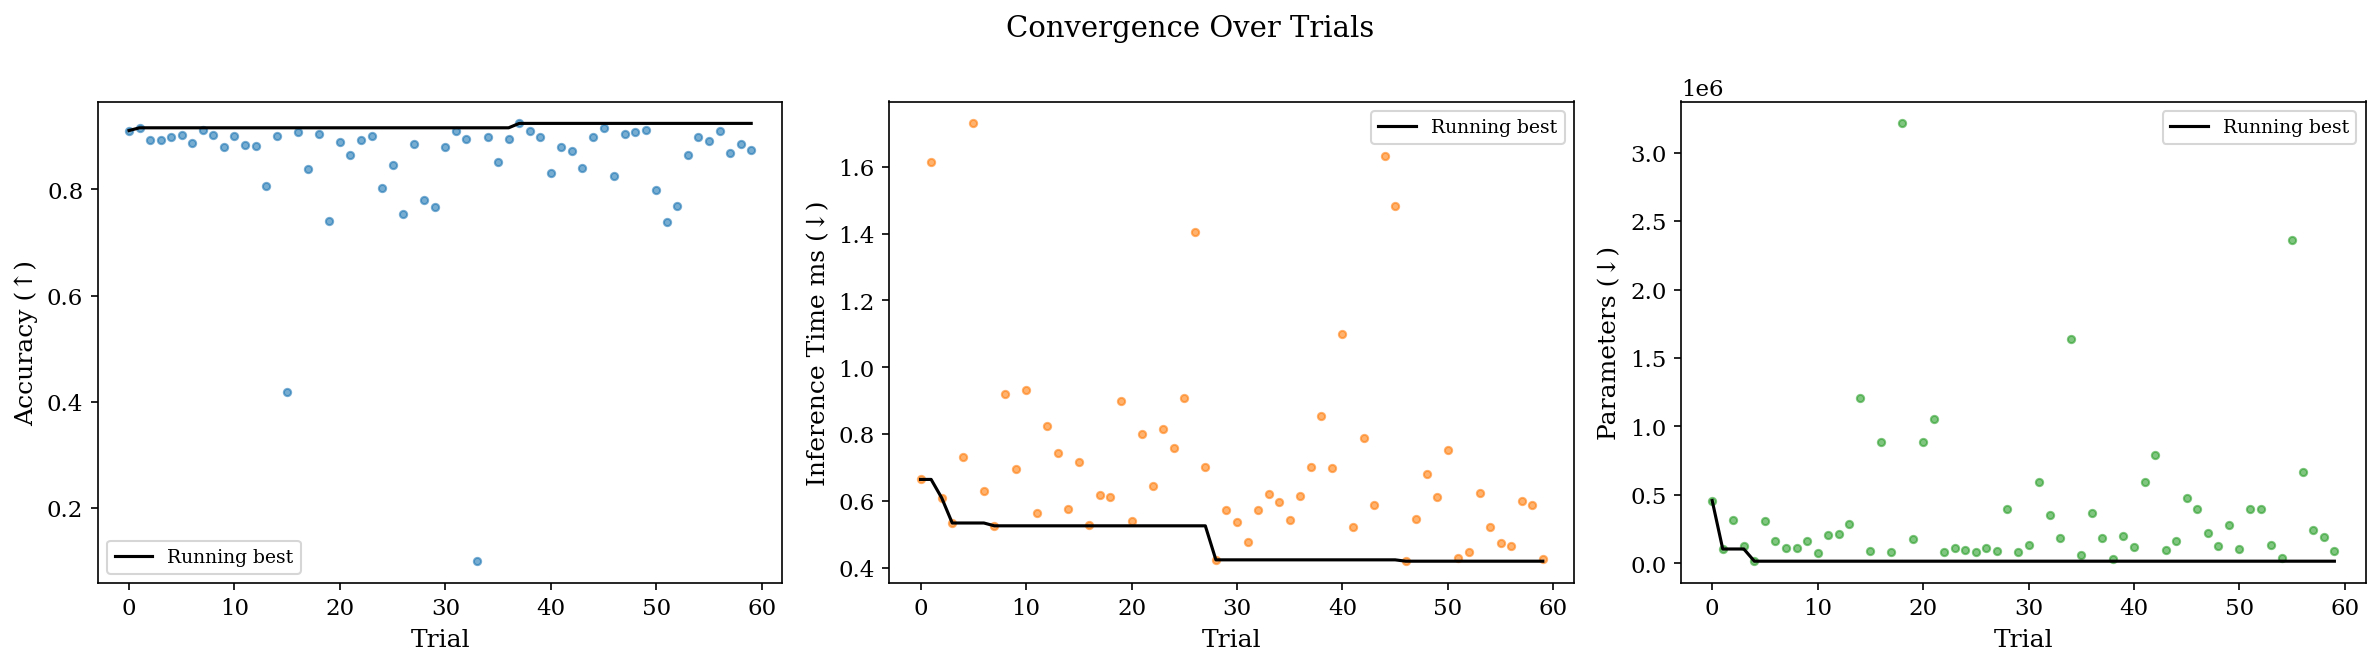
\includegraphics[width=\textwidth]{figures/convergence.png}
\caption{Convergence plots showing individual trial values and running
best for accuracy, inference time, and parameter count.}
\label{fig:convergence}
\end{figure}

\subsection{Hyperparameter Distribution}

Figure~\ref{fig:params} compares the distribution of categorical
hyperparameters between all evaluated trials and Pareto-optimal solutions.

\begin{figure}[H]
\centering
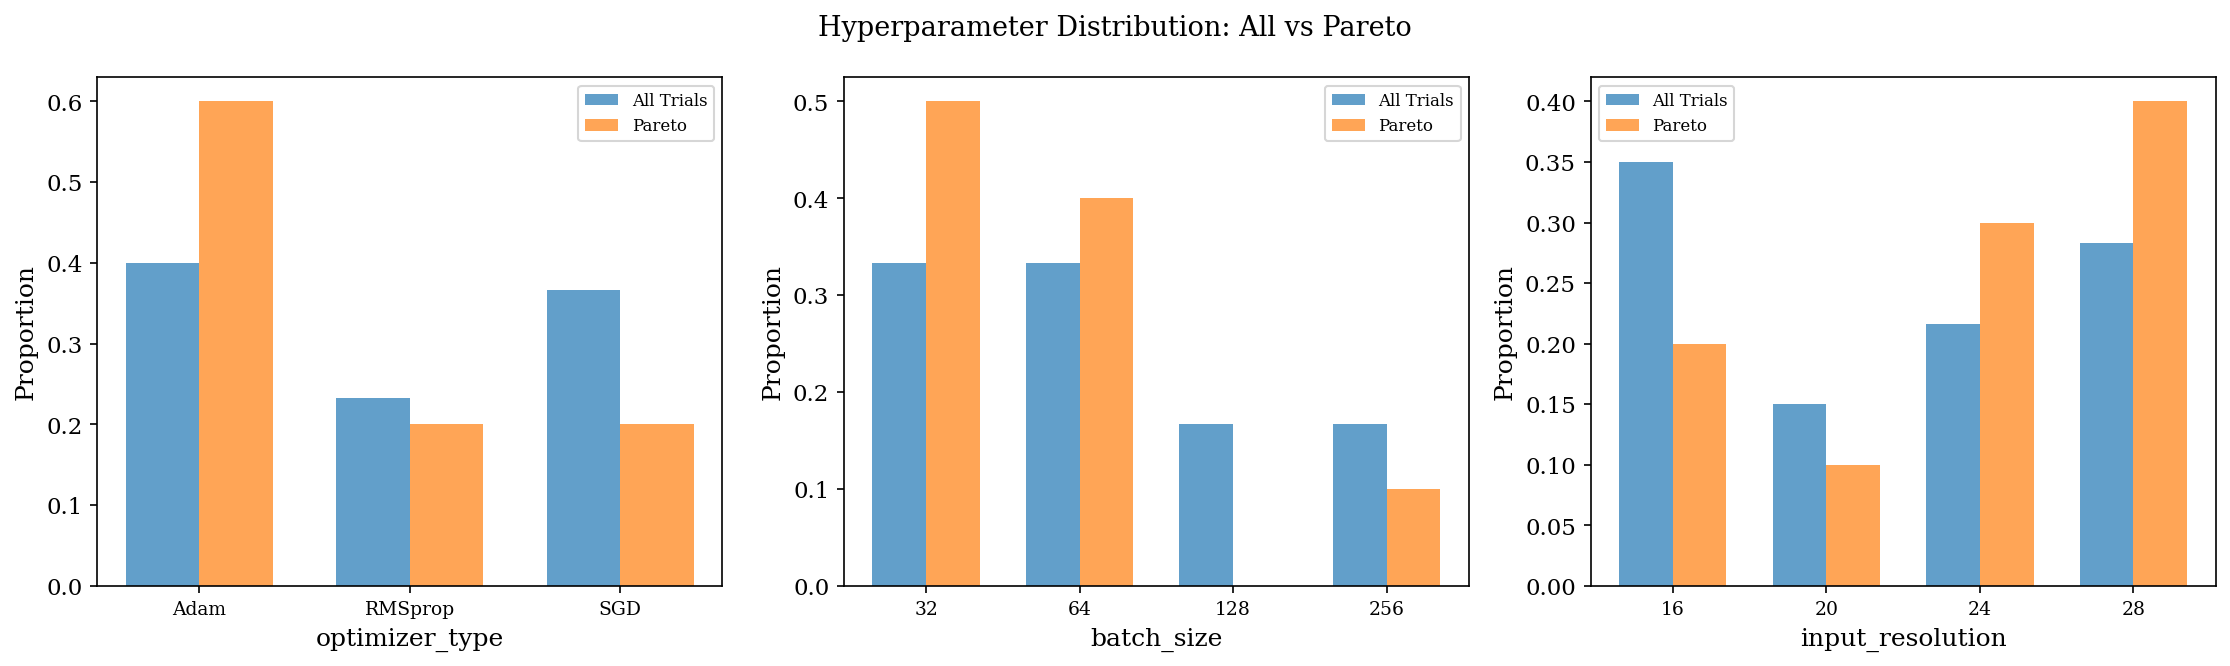
\includegraphics[width=\textwidth]{figures/param_distribution.png}
\caption{Hyperparameter distribution: All trials vs.\ Pareto-optimal solutions.}
\label{fig:params}
\end{figure}

\subsection{Pareto Front Tabulation}

Table~\ref{tab:pareto} lists all Pareto-optimal solutions, sorted by
classification accuracy.

% This table is auto-generated by analyze_results.py
\begin{table}
\caption{Pareto-optimal solutions sorted by accuracy.}
\label{tab:pareto}
\begin{tabular}{cccc}
\toprule
trial & accuracy & inference_ms & n_parameters \\
\midrule
37 & 0.9243 & 0.7027 & 182714 \\
1 & 0.9160 & 1.6141 & 104570 \\
7 & 0.9118 & 0.5261 & 109066 \\
38 & 0.9096 & 0.8547 & 33370 \\
56 & 0.9092 & 0.4643 & 666122 \\
31 & 0.9091 & 0.4784 & 591626 \\
54 & 0.8986 & 0.5234 & 42218 \\
4 & 0.8984 & 0.7305 & 15370 \\
59 & 0.8748 & 0.4273 & 86250 \\
46 & 0.8248 & 0.4203 & 395210 \\
\bottomrule
\end{tabular}
\end{table}


\subsection{Quality Metrics}

\begin{table}[H]
\centering
\caption{Pareto front quality metrics.}
\label{tab:metrics}
\begin{tabular}{@{}lrl@{}}
\toprule
\textbf{Metric} & \textbf{Value} & \textbf{Interpretation} \\
\midrule
Hypervolume         & 11{,}128.77 & Volume dominated by the Pareto front; higher is better \\
Spacing ($S$)       & 0.2155      & Distribution uniformity; lower means more uniform \\
Spread ($\Delta$)   & 42.60       & Extent of the front; higher means wider coverage \\
$|\mathcal{P}^*|$   & 10          & Number of non-dominated solutions out of 60 trials \\
\bottomrule
\end{tabular}
\end{table}

The hypervolume of 11{,}128.77 indicates substantial coverage of the
objective space. The spacing metric of 0.2155 suggests a reasonably
uniform distribution of solutions along the Pareto front. The 10
non-dominated solutions (out of 60 total trials) represent a 16.7\%
Pareto-optimality rate, providing a diverse set of trade-off
configurations for the decision-maker.

% ====================================================================
\section{Trade-off Analysis}
\label{sec:tradeoffs}

\subsection{Accuracy vs.\ Model Size}
Larger models with more convolutional layers and wider channels achieve
higher accuracy, but with diminishing returns. Trial~37 achieves the
highest accuracy (92.43\%) with 182{,}714 parameters, while Trial~4
achieves 89.84\% with only 15{,}370 parameters — a 12$\times$ reduction
in size for merely 2.6\% accuracy loss. Meanwhile, Trial~56 uses
666{,}122 parameters (the largest Pareto-optimal model) but achieves only
90.92\% accuracy, indicating that simply scaling parameters does not
guarantee proportional accuracy gains.

\subsection{Accuracy vs.\ Inference Time}
Inference time is influenced by both model depth and input resolution.
The fastest Pareto-optimal model (Trial~46, 0.42\,ms) uses resolution
$16\times16$ but achieves only 82.48\% accuracy. In contrast, Trial~37
(0.70\,ms, 92.43\%) uses full $28\times28$ resolution. The ``knee''
solutions — Trials~7 and 54 — offer approximately 90\% accuracy at
0.52\,ms, representing practical trade-offs for latency-sensitive
deployments.

\subsection{Model Size vs.\ Inference Time}
Interestingly, model size and inference time are not strictly correlated
in our Pareto front. Trial~31 has 591{,}626 parameters but only 0.48\,ms
inference time (1 conv layer), while Trial~4 has 15{,}370 parameters but
0.73\,ms inference (4 conv layers). This shows that \emph{depth} affects
latency more than \emph{width}, since deeper models require sequential
computation while wider layers can be parallelized on GPU.

\subsection{Practical Recommendations}
Based on the Pareto front, we identify three deployment scenarios:
\begin{description}
    \item[High Accuracy ($>$92\%):] Trial~37 — 3 conv layers, 28$\times$28
    input, Adam optimizer, 182K parameters. Best for server-side deployment.
    \item[Balanced ($\sim$90\%, fast):] Trial~7 — 3 conv layers, 20$\times$20
    input, Adam, 109K parameters, 0.53\,ms. Ideal for most applications.
    \item[Edge / Minimal ($<$90\%, ultra-light):] Trial~4 — 4 conv layers
    (narrow), 24$\times$24, RMSprop, only 15K parameters. Suitable for
    mobile and IoT deployment.
\end{description}

% ====================================================================
\section{Discussion}
\label{sec:discussion}

\subsection{Key Insights}
\begin{enumerate}
    \item NSGA-II effectively discovers 10 diverse non-dominated solutions
    across the 3-objective space in just 60 trials, achieving a Pareto-optimality
    rate of 16.7\%.
    \item The number of convolutional layers and channel width are the
    most influential architectural decisions — accuracy ranges from
    82.48\% to 92.43\% across the Pareto front.
    \item Input resolution acts as a ``meta-parameter'' that trades
    spatial information for speed: reducing from $28\times28$ to
    $16\times16$ reduces inference time by $\sim$40\% but costs
    $\sim$5--10\% accuracy.
    \item Adam optimizer dominates the Pareto front (7 of 10 solutions),
    suggesting it is the most robust optimizer across diverse architectures.
    \item Model depth affects inference latency more than model width,
    as observed in the size-vs-time analysis.
\end{enumerate}

\subsection{Limitations}
\begin{itemize}
    \item Training is limited to 3--15 epochs; some configurations may
    benefit from longer training.
    \item Inference time measurements can be noisy on shared hardware.
    \item The search space is manually defined; automated architecture
    search could explore richer spaces.
    \item Only Fashion-MNIST is evaluated; generalization to other
    datasets is not tested.
\end{itemize}

\subsection{Future Work}
\begin{itemize}
    \item Extend to NSGA-III for better many-objective scaling.
    \item Include FLOPs as a fourth objective.
    \item Apply transfer learning from pre-trained models.
    \item Evaluate on CIFAR-10/100 and medical imaging datasets.
\end{itemize}

% ====================================================================
\section{Conclusion}
\label{sec:conclusion}

We presented a multi-objective optimization framework for CNN
hyperparameter tuning, jointly optimizing classification accuracy,
inference time, and model size on Fashion-MNIST. Using NSGA-II via
Optuna, we identified a diverse Pareto front of non-dominated solutions.
The trade-off analysis reveals that moderate architectures (2--3
convolutional layers, 32--64 channels) offer compelling accuracy--efficiency
trade-offs. The hypervolume, spacing, and spread metrics confirm the
quality and diversity of the discovered Pareto front. This framework
enables practitioners to make informed, deployment-aware model selection
decisions.

% ====================================================================
\begin{thebibliography}{9}

\bibitem{deb2002fast}
K.~Deb, A.~Pratap, S.~Agarwal, and T.~Meyarivan,
``A fast and elitist multiobjective genetic algorithm: NSGA-II,''
\emph{IEEE Trans.\ Evolutionary Computation}, vol.~6, no.~2,
pp.~182--197, 2002.

\bibitem{xiao2017fashion}
H.~Xiao, K.~Rasul, and R.~Vollgraf,
``Fashion-MNIST: a novel image dataset for benchmarking machine learning
algorithms,'' \emph{arXiv preprint arXiv:1708.07747}, 2017.

\bibitem{optuna}
T.~Akiba, S.~Sano, T.~Yanase, T.~Ohta, and M.~Koyama,
``Optuna: A next-generation hyperparameter optimization framework,''
in \emph{KDD}, 2019.

\bibitem{zitzler2003}
E.~Zitzler, L.~Thiele, M.~Laumanns, C.~M.~Fonseca, and V.~G.~da~Fonseca,
``Performance assessment of multiobjective optimizers: An analysis and
review,'' \emph{IEEE Trans.\ Evolutionary Computation}, vol.~7, no.~2,
pp.~117--132, 2003.

\bibitem{schott1995}
J.~R.~Schott,
``Fault tolerant design using single and multicriteria genetic algorithm
optimization,'' M.S.~thesis, MIT, 1995.

\end{thebibliography}

\end{document}
